\section{Security Framework Model}

%In this section, we begin by explaining the security policy model of
%DASF that we designed. Afterward, we focus on
%the architecture and implementation of the DASF prototype on Android.

%\subsection{Security Model}

On an Android device, there are
a set of applications, $A := \left\{a_{1},a_{2},\ldots,a_{n}\right\}$.
Each application, $\forall a_{i} \in A$, where $1 \le i \le n$,
contains a set of permissions that the application requests,
$P_{a_{i}} := \left\{p_{1}, p_{2},\ldots,p_{m}\right\}$,
and a set of components,
$C_{a_{i}} := \left\{c_{1},c_{2},\ldots,c_{q}\right\}$.
Each application is either a system application, $S_{A}$,
or a third-party application, $T_{A}$, such that $S_{A}\subset A$, and $T_{A} \subset A$,
but $S_{A} \cap T_{A} = \left\{\right\}$.

\subsection{Dynamic Privilege Restriction Security Policy.}  

A permission, $p$, is restricted if the restricted permission, denoted
as $R\left(p\right)$, is imposed
by a specific application $a_{i}$.
%such that $a_{j} \in A$ and $1 \le j \le m$.  
In Android, permissions are granted at the granularity
of the entire application.  If the permissions of a specific
application, $a_i$, is granted, its corresponding components,
$C_{a_i}$ are allowed to be launched. Obviously, for any application
that can successfully run, each of its components has to have the
permission to be launched. We use $L(C_{a_i})$ to
denote the launching of $a_i$'s components: $c_1, c_2,...,c_q$.
%
%Since permissions are granted at the granularity
%of the entire application rather than at the granularity of its individual
%components, the application's components that are permitted
%to be launched is denoted as $L\left(C_{a_{i}}\right)$. This means,
%$\forall c_{k} \in C_{a_{i}} : L\left(c_{k}\right)$ such that 
%$1 \le k \le o$.  
Furthermore, we denote killing the process
that an application, $a_{i}$, is running under as $K(a_{i})$.

Therefore, the security policy for an application is a procedure of
imposing the restricted permissions which determine whether or not the
application and its components can be launched. Given an application
$a_i$, its components launching, $L(C_{a_i})$, will be
successful as long as one the security policy satisfy any one of the
following conditions:

\[\left\{
\begin{array}{l}
a_i \in S_A\\
%a_i \in T_A \wedge R\left(p\right) \wedge p \in P_{a_{i}} \\
%\wedge a_i = a_j\\
a_i \in T_{A} \wedge \lnot R\left(p\right) \wedge p \in P_{a_{i}}.\\
\end{array}
\right.
\]


%for starting an application, $a_{i}$,
%and it's components, $C_{a_{i}}$, is defined as follows.

%$a_{i} \in S_{A} \to L\left(C_{a_{i}}\right)$

%$a_{i} \in T_{A} \wedge R\left(p\right) \wedge p \in P_{a_{i}} \wedge a_{i} = a_{j} \to L\left(C_{a_{i}}\right)$

%$a_{i} \in T_{A} \wedge \lnot R\left(p\right) \wedge p \in P_{a_{i}} \to L\left(C_{a_{i}}\right)$

\begin{comment}
$a_{i} \in T_{A} \wedge R\left(p\right) \wedge p \in P_{a_{i}} \wedge a_{i} \neq a_{j} \to \lnot L\left(C_{a_{i}}\right)$
\end{comment}
More significantly, DASF is able to impose the
policy on application that are already running when a permission is
dynamically restricted for a security purpose.  In that case, any
running application $a_i$ with the following updated policy:
\[\left.
\begin{array}{l}
(a_{i} \in T_{A}) \wedge R\left(p\right) \wedge (p \in P_{a_{i}})\\
\end{array}
\right.
\]
will lead to $K(a_i)$, i.e., be terminated.  And the running
application status with the following
new policy, $ a_{i} \in T_{A} \wedge \lnot R\left(p\right) \wedge p \in P_{a_{i}}$,
%\[\left \{
%\begin{array}{l}
%a_{i} \in S_{A}\\
%a_{i} \in T_{A} \wedge \lnot R\left(p\right) \wedge p \in P_{a_{i}} \wedge a_{i} = a_{j}\\
%\end{array}
%\right.
%\]
will become $\lnot K(a_i)$, i.e., not be affected.
%Moreover, the security policy imposed on applications that are 
%already running when a permission is dynamically restricted
%is defined as follows.

%$a_{i} \in S_{A} \to \lnot K\left(a_{i}\right)$

%$a_{i} \in T_{A} \wedge \lnot R\left(p\right) \wedge p \in P_{a_{i}} \wedge a_{i} = a_{j} \to \lnot K\left(a_{i}\right)$


%$a_{i} \in T_{A} \wedge R\left(p\right) \wedge p \in P_{a_{i}} \to K\left(a_{i}\right)$

In other words, an application's components are always allowed to
start if they belong to a system application.  Moreover, system
applications are never forcibly closed if a permission is dynamically
restricted.  If the application is a third-party application, however,
the following policies are enforced. First, a third-party
application's components are not permitted to start if the application
requests a permission that is currently restricted and the application
is not the one that imposed the permission restriction.  Second, a
third-party application's components are permitted to start if the
application does not request any permissions that are currently
restricted. Furthermore, if a permission is dynamically restricted and
a third-party application that is currently running has requested that 
permission and was not the application that imposed the permission
restriction, the application will be forcibly closed.

%Since DASF provides support for a certified~\footnote{The
%  certification process can be dictated by the organization, e.g., a
%  hospital, throught an out-of-band channel.} third-party
%applications to programmatically restrict permissions, the
%application, $a_{i}$, must define a set of permissions that it is
%permitted to restrict, $X_{a_i} := {p_1, p_2,\ldots,p_m}$,
%during the application's installation and approved by the user to prevent
%the abuse of dynamic permission restrictions.  Thus, a third-party application,
%$a_{i}$, is allowed to restrict a permission, $p$, if $p \in X_{a_{i}}$.

\subsection{Security Policies on Sensitive Data.}
A mobile device contains a set of data (e.g., strings, integers, arrays,
etc.) in RAM, $\left\{d_{1},d_{2},\ldots,d_{n}\right\}$,
each of which has its corresponding sensitivity level. In our
framework, we use a privacy tag, $T(d_i)$, with the possible values of
$\left\{t_{1},t_{2},\ldots,t_{m}\right\}$, to represent data $d_i$'s
sensitivity level.
%$\left\{t_{1},t_{2},\ldots,t_{m}\right\}$, to represent a variety of 
%sensitivity levels.  
%privacy tag: $T(d_i)$, where $1\leq i\leq n$. 
%Since we utilize the dynamic taint tracking system provided
%by TaintDroid, each element in the set of data also includes
%a privacy tag, $T\left(d_{i}\right)$, which denotes the data's sensitivity level
%that comes from the set of possible privacy tags,
%$\left\{t_{1},t_{2},\ldots,t_{m}\right\}$.
%%
%
%Thus, we denote the set of data in the Java stack as a set
Thus, we can denote the data set as a set containing a privacy tag and
the data:
%containing a privacy tag and the data,
$D := \left\{\left\{d_{1}, T\left(d_{1}\right)\right\},\left\{d_{2},T\left(d_{2}\right)\right\},\ldots,\left\{d_{n},T\left(d_{n}\right)\right\}\right\}$.

It is possible for two pieces of data, $d_{j}$, $d_{k}$, where $1 \le
j \le n$ and $1 \le k \le n$,  with different privacy tags
to be combined (e.g., concatenating two strings with different
sensitivity levels).  The general propagation rules of the
privacy tags are as follows when data with two different privacy tags
are combined:

$T(d_{j}) \ge T(d_{k}) \to T(d_{j}\wedge d_{k}) = T(d_{j})$,

$T(d_{j}) < T(d_{k}) \to T(d_{j} \wedge d_{k}) = T(d_{k})$.

These propagation rules ensure that when two pieces of
data are combined, the highest sensitivity level is propagated
to the combined data.   This means that if the sensitivity
level of $d_{j}$ is greater than or equal to the sensitivity
level of $d_{k}$, the combined data has the sensitivity level
of $d_{j}$.  Further, if the sensitivity level of $d_{j}$ is
less than the sensitivity level of $d_{k}$, the combined data
has the sensitivity level of $d_{k}$.

We define two operations on the data that our security policy
must handle.  First, $W(d_{j})$, denotes writing the data to
flash memory (e.g., to a file or an SQLite database). Second,
$F(d_{j})$ denotes forwarding the data from the device
(e.g., through a socket, bluetooth socket, SMS, and MMS).
Furthermore, data, $d_{j}$, that can either be forwarded from the
device or written to flash memory is denoted as $FW\left(d_{j}\right)$.
The operations that are permitted on the data are determined by the
data's privacy tag.  The privacy tag, $t_0$, denotes
that $T(d_{j}) = t_0 \to \lnot FW\left(d_{j}\right)$. The privacy tag,
$t_1$, denotes $T(d_{j}) = t_1\lnot W\left(d_{j}\right)$.  Finally,
the privacy tag, $t_2$, denotes 
$T(d_{j}) = t_2 \to \lnot F\left(d_{j}\right)$.  Furthermore, we reserve
the privacy tag, $t_m$, to denote sensitive information that have
no security policies enforced by the system.  The value of $m$ is a
system parameter and can be adjusted depending on the requirement of
the security levels. 

To ensure that the security policies are enforced correctly when
combining two pieces of data with different sensitivity levels,
the propagation rules of the data's sensitivity levels must
include an escalation of sensitivity levels.  For example, if
data with the privacy tag $t_1$ is combined with data with
the privacy tag $t_2$, the combined data should have the
privacy tag $t_0$ rather than $t_1$ or $t_2$.  Thus, the propagation
of privacy tags are adjusted as follows when data is combined:

$T\left(d_{j}\right) = t_1 \wedge T\left(d_{k}\right) = t_2 \to T\left(d_{j}+d_{k}\right) = t_0$.

This propagation rules ensures that if data that is restricted from
being forwarded from the device is combined with data the is restricted
from being written to flash memory, the combined data will be restricted
from being written to the flash memory and forwarded from the device.

\subsection{Application-Layer Message Protocol.}   
DASF also includes an application-layer message protocol
that allows a server to dynamically enforce privilege restrictions
on the device and enforce the previously mentioned security policies
on data that is sent to the device.  The message
protocol assumes that it is built over an SSL connection to ensure
a secure communication channel between the client (e.g., mobile
device) and the server.

The message protocol consists of applications sending a request to
the server (e.g., requesting data) and the server responding back
to the request (e.g., sending the data).  The message protocol
allows the server to impose a sensitivity level on the data in
its response, and thus, impose a security policy on the data that
it sends to the client.  We call the server responding to the
client's request for data as a \textit{data message}.
The header of the \textit{data message} denotes the type of message,
sensitivity level, and the length of the payload.  The contents of a
\textit{data message} is shown in Fig.~\ref{fig:datamessage}.

\begin{figure}[ht]
\centering
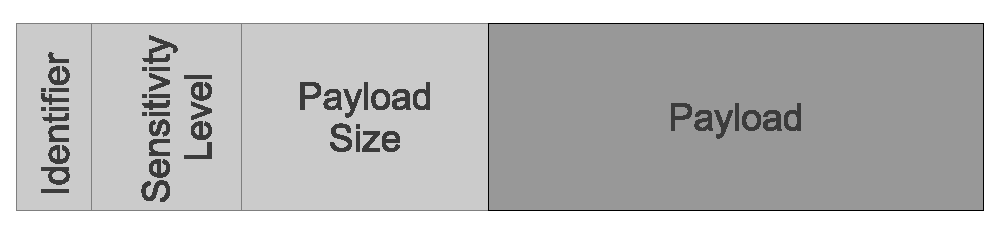
\psfig{file=data_message.eps, width=2.5in}
\caption{Data Message}
\label{fig:datamessage}
\end{figure}

%\vspace{-3mm}

When an application requests data from the server, the server
responds back to the client with
$data\_message\left(\left\{sensitivity\_level, response\right\}\right)$.
The system extracts sensitivity level and applies that sensitivity level
to the response before passing it to the application.  The sensitivity
level, $s$, corresponds to one of the four privacy tags that we previously defined.
For example,  $s \in \left\{t_m,..., t_2, t_1, t_0\right\}$.

The server can also dynamically impose any privilege restrictions on
the device without asking the user for permission.  To prevent the
abuse of server-imposed privilege restrictions, the application must
be declared as a \textit{medical application} during its installation
and the system insures that the client application connects to the
organization's trusted server. The above assurance is achieved by a
server-side periodic encrypted heartbeat message that confirms the
application's aliveness.  Note that under our security framework, the
connection between the server and the \textit{medical application} is
supposed to be persistent; the tear-down of the connection will lead
to the termination of the application due to the security concern. 
The system secret key update and the privilege control message
(as described below) can be arranged as a piggyback in the heartbeat 
messages.  
%The server may dynamically impose
%privilege restrictions, or unrestricted previously imposed privilege
%restrictions, on the device by prepending a
%\textit{privilege control message} to the \textit{data message}.

The dynamic security provisioning is enforced by the \textit{privilege
  control message}, which must be encrypted with a one-time key so
that DASF can verify that the policy originated from the server and to
prevent replay attacks. The one-time key can be provided by a server
generated one-way key chain, similar to S/Key mechanism~\cite{skey}. 
Our security framework fetches the initial master secret key from the
server when the device is first booted and updates the master key, if
necessary, through the server heartbeat message as described above. 
%
%Furthermore, the payload of the \textit{privilege control message} must be
%encrypted using a one-time key to prevent applications from abusing
%this functionality.  The payload must be encrypted with a one-time
%key so that DASF can verify that the policy
%originated from the server and to prevent replay attacks.  Our
%security framework fetches the initial secret key from the server
%when the device is first booted.
%
%The payload of the \textit{privilege control message} contains a list
%of privilege restrictions, privilege unrestrictions, and a new secret
%key.  
%The entire payload is encrypted using the previous key,
%$E\left(key, payload\right)$.  
The header of the \textit{privilege control
 message} contains the type of message, a flag denoting that a data message
is appended, and the length of the payload. The contents of 
a \textit{privilege control message} is shown in
Fig.~\ref{fig:privilegemessage}.  When the system receives a
\textit{privilege control message}, it passes the payload to DASF.
If the security framework successfully decrypts
the payload, $D\left(key, payload\right)$, the set of permission restrictions
and unrestrictions are imposed and the secret key is updated.

\begin{figure}[ht]
\centering
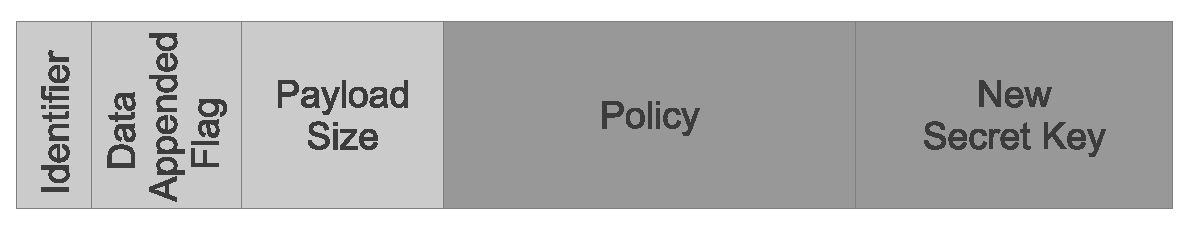
\psfig{file=policy_message.eps, width=2.5in}
\caption{Privilege Control Message}
\label{fig:privilegemessage}
\end{figure}

